\begin{frame}
  \frametitle{Depósitos del Tesoro Nacional}
  \begin{center}
    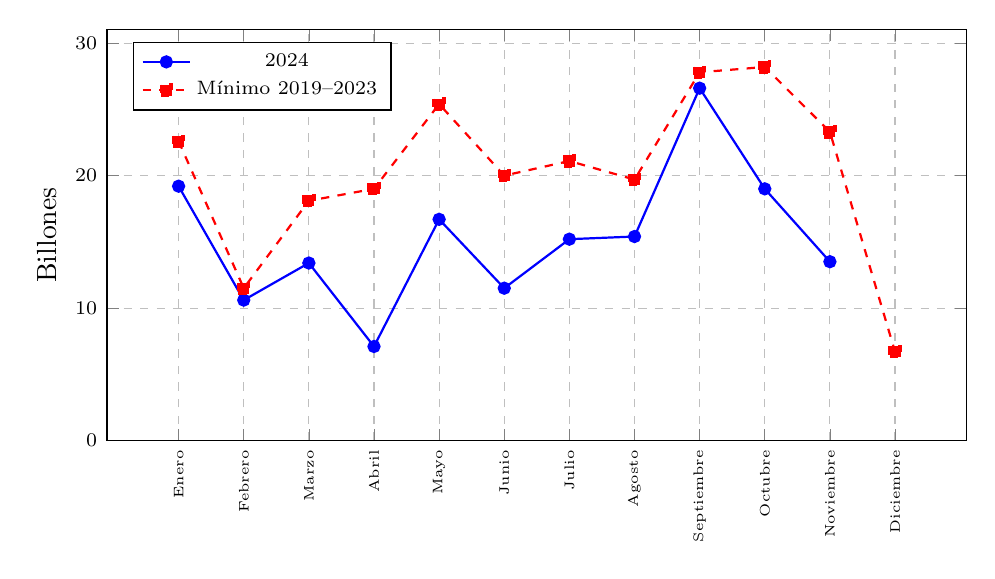
\begin{tikzpicture}
    \begin{axis}[
        width=12.5cm,
        height=6.8cm,
        ylabel={Billones},
        xtick={1,2,3,4,5,6,7,8,9,10,11,12},
        xticklabels={Enero,Febrero,Marzo,Abril,Mayo,Junio,Julio,Agosto,Septiembre,Octubre,Noviembre,Diciembre},
        xticklabel style={rotate=90, anchor=east, font=\tiny},
        yticklabel style={font=\scriptsize},
        grid=both,
        grid style=dashed,
        ymin=0,
        legend pos=north west,
        legend style={font=\scriptsize}
    ]

    % Serie 2024
    \addplot[mark=*, thick, blue] coordinates {
        (1,19.2) (2,10.6) (3,13.4) (4,7.1) (5,16.7) (6,11.5) 
        (7,15.2) (8,15.4) (9,26.6) (10,19.0) (11,13.5)
    };
    \addlegendentry{2024}

    % Mínimos históricos
    \addplot[mark=square*, color=red, thick, dashed] coordinates {
        (1,22.6) (2,11.5) (3,18.1) (4,19.0) (5,25.4) (6,20.0) 
        (7,21.1) (8,19.7) (9,27.8) (10,28.2) (11,23.3) (12,6.7)
    };
    \addlegendentry{Mínimo 2019–2023}

    \end{axis}
    \end{tikzpicture}

    \vspace{0.2cm}
    \scriptsize\textit{Fuente: Cálculos con base en datos de la Dirección de Crédito Público, Ministerio de Hacienda.}
  \end{center}
\end{frame}
